%%%%%%%%%%%%%%%%%  Debut du fichier Latex  %%%%%%%%%%%%%%%%%%%%%%%%%%%%%%
\documentclass[a4paper,12pt,onecolumn]{article}

%%% Pour un texte en francais

%%\usepackage[applemac]{inputenc}
%\usepackage[francais]{babel}
	         % encodage des lettres accentuees
\usepackage[T1]{fontenc}
\usepackage[utf8]{inputenc}          % encodage des lettres accentuees
%\usepackage{graphicx}
%%\usepackage{graphicx} \def\BIB{}
\usepackage[paper=a4paper,textwidth=140mm,left=2.5cm,right=2.5cm,top=3cm,bottom=3cm]{geometry}
\usepackage{multicol}
\usepackage{graphicx,wrapfig,lipsum} 
%\def\BIB{}
\usepackage[font=footnotesize]{caption}
\usepackage{subcaption}
\usepackage[pdftex]{hyperref}
\usepackage{natbib}
\usepackage{url}
\usepackage{perpage} %the perpage package
\MakePerPage{footnote} %the perpage package command
\hypersetup{
    colorlinks,%
    citecolor=black,%
    filecolor=black,%
    linkcolor=black,%
    urlcolor=blue     % can put red here to visualize the links
}


\DeclareUnicodeCharacter{00A0}{ }

%%% Quelques raccourcis pour la mise en page
\newcommand{\remarque}[1]{{\small \it #1}}
\newcommand{\rubrique}{\bigskip \noindent $\bullet$ }

\newcommand{\ignore}[1]{}

\renewcommand*\rmdefault{iwona}

\pagenumbering{gobble}

%\bibliographystyle{abbrvnat}
%\setcitestyle{authoryear,open={((},close={))}}

%\renewcommand{\thefootnote}{\roman{footnote}}

% -------------------------------------------------
\newcommand{\horrule}[1]{\rule{\linewidth}{#1}} % Create horizontal rule command with 1 argument of height

\title{	
\vspace*{-2cm}
\normalfont \tiny 
%\textsc{Paris Diderot} \\ [25pt] % Your university, school and/or department name(s)
\horrule{0.5pt} \\[0.4cm] % Thin top horizontal rule
\huge Research statement \\ % The assignment title
\horrule{2pt} \\[0.5cm] % Thick bottom horizontal rule
}
\author{El Mellah Ileyk} % Your name
\date{\tiny }%\normalsize\today} % Today's date or a custom date
% -------------------------------------------------

%\makeatletter
%\def\@xfootnote[#1]{%
%  \protected@xdef\@thefnmark{#1}%
%  \@footnotemark\@footnotetext}
%\makeatother

\begin{document}

%\bibpunct{[}{]}{;}{n}{,}{,}

%%%%%%%%%%%%%%%%%%%%%%%%%  PREMIERE PAGE %%%%%%%%%%%%%%%%%%%%%%%%%%%%%%
%%% DANS CETTE PAGE, ON REMPLACE LES INDICATIONS ENTRE CROCHETS [...]
%%% PAR LES INFORMATIONS DEMANDEES
%%%%%%%%%%%%%%%%%%%%%%%%%%%%%%%%%%%%%%%%%%%%%%%%%%%%%%%%%%%%%%%%%%%%%%%

\maketitle
\thispagestyle{empty}

X-ray emitting binary systems host a compact object - a neutron star (NS) or a black hole (BH) - orbiting a stellar companion whose gas is accreted by the former. Since the discovery of the first extrasolar X-ray source in the early sixties \citep{Giacconi1962}, continuous observations of those systems have revealed a broad range of spectral and photometric behaviors with a special emphasis on their incredible time variability : flares, hysteresis loops in hardness-luminosity diagrams, off-states, quasi-periodic oscillations... all this on time scales ranging from milliseconds to years, fully within the scope of observational missions lifetimes (XMM-Newton, Chandra and Integral today, SVOM, LOFT and Athena tomorrow). The complex Physics at stake behind the scenes has long been beyond our reach due to limited observational data and numerical capacities. Those intrinsically intertwined systems require multi-scales approaches to fully appreciate the turbulent flow, from the Dantean stellar surface up to the magnetic vicinity of a NS, if not the relativistic surroundings of a BH. Game changing high performance computing technologies have ushered in a gold rush to design coupled semi-analytical models supported by numerical simulations to account for time variability in X-ray binaries. Once pie in the sky, a consistent overview of the accretion process is now within our grasp.

\subsection*{Past activity}

\subsubsection*{PhD research activity}

\begin{figure}[!b]
\begin{center}
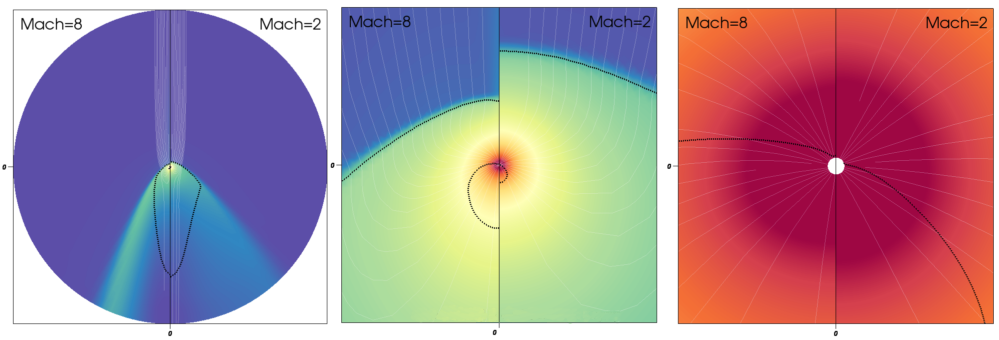
\includegraphics[height=5.5cm, width=16cm]{Figures/zoom_BHL.png}	
\caption{Successive zoom in on the innermost parts of a planar flow (coming from the top) being deflected by a central accretor for different Mach numbers at infinity. In white are represented the streamlines while the the dotted black lines represent the Mach=1 surfaces.}
\label{fig:zoom_BHL}
\end{center}
\end{figure}

\indent During my 3 years of PhD, I concentrated on mass transfer in binaries via wind accretion, the low angular momentum counterpart of the more comprehensively understood Roche lobe overflow (RLOF) mechanism. Supergiant X-ray binaries (SgXB), where a compact object (generally a NS) orbits an evolved O/B supergiant, are the ideal stage for wind accretion to occur. Indeed, the latter displays intense outflows, a fraction of which being captured by the NS. The rapid increase since the late 2000’s in the number of SgXB \citep{Walter15} and the ambiguous status of the newly discovered SFXTs \citep{Negueruela2006} only increased the appeal of this burning topic.\\ \\
\indent In a first attempt to better understand the wind accretion process, I confronted the analytical prescriptions given by Bondi, Hoyle and Lyttleton \citep[BHL,][]{Hoyle:1939fl,Bondi1944} to a hydrodynamical (HD) representation of the flow. To do so, I used and developed the explicitely flux-conserving finite volume transport code \texttt{MPI-AMRVAC}, a code whose origins trace back to the mid 90’s when G\'abor T\'oth and Rony Keppens first tackled the question \citep{Toth1996,Toth1998}. The new version I contributed to now addresses hydrodynamical or magneto-hydrodynamical problems, in Cartesian, cylindrical or spherical geometry, with or without polytropic prescriptions, source terms, etc \citep{Xia2017}. For wind speeds similar to the ones observed in SgXB ($\sim$1,000km$\cdot$s$^{-1}$), the main challenge is the contrast between the scale at which the gravitational beaming of the fast inflow by the accretor becomes significant (the accretion radius) and the size of the compact accretor, typically 4 to 5 orders of magnitude smaller. Since most of the emitted light comes from the immediate vicinity of the accretor, it is important to follow the flow through these scales. To uniformly resolve the incoming planar flow, I implemented a radially stretched grid in a 2D spherical geometry. With suitable boundary conditions, I reached a numerically relaxed state and spanned the 5 required orders of magnitude thanks to the computing time I was granted on the CINES Tier-1 cluster (see Figure\,\ref{fig:zoom_BHL}). In \cite{ElMellah2015}, I characterized the structure of the flow, which forms a stable detached bow shocked as it is beamed towards the wake of the accretor, and the dependence of the mass accretion rate on the Mach number of the inflow. For the first time, we monitored the flow deep enough to also confirm the analytical prediction by \cite{Foglizzo1997} concerning the topology of the inner sonic surface (where the shocked flow becomes supersonic again) which has to be anchored into the accretor.\\ \\
\indent In a realistic SgXB though, the incoming wind is not planar due to the orbital effects. It carries a non-zero angular momentum which could, in some cases, lead to the formation of a wind-capture disc. To identify the favorable configurations, I designed a model of supersonic line-driven wind propagation in SgXB, coupling the stellar, orbital, wind and accretion parameters \citep{ElMellah2016a}. I identified the minimal set of dimensionless degrees of freedom of the problem to optimally explore the space of parameters. This investigation showed how sheared and beamed the wind is when it enters the region around the accretor where the shock is expected to develop - i.e. where the ballistic assumption breaks up and where HD simulations similar to the ones above are required. The need to connect the orbital scale motion, essentially ballistic, and the accretion region, centered on the compact object, became apparent.\\

\subsubsection*{Postdoctoral research activity}

\begin{figure}[!b]
\begin{subfigure}{0.45\columnwidth}
  \centering
%  \hspace*{-1cm}
  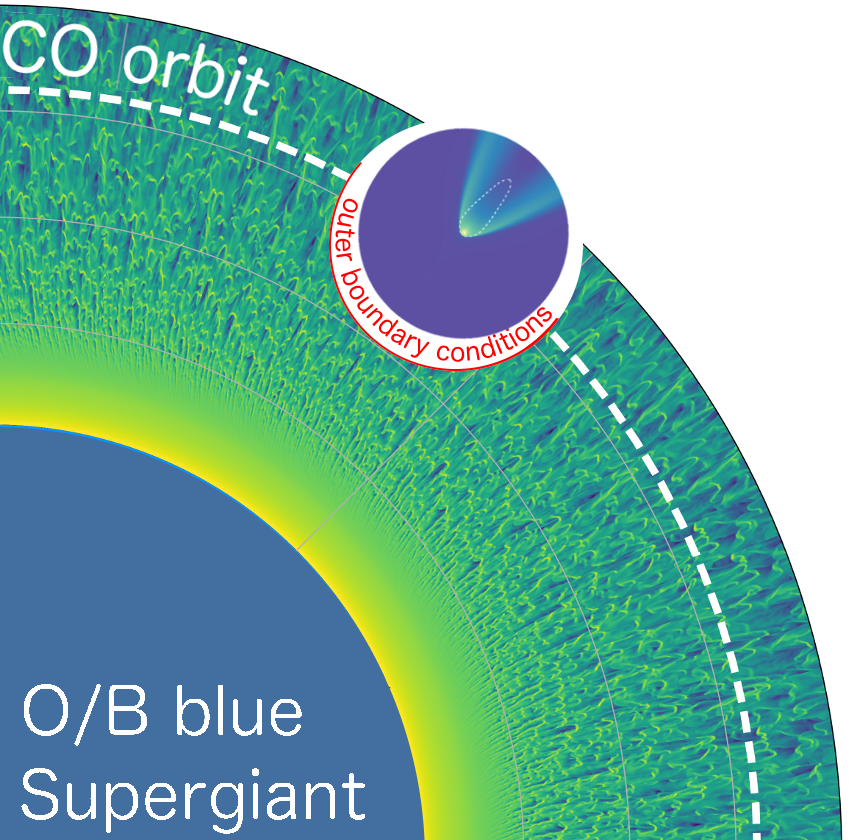
\includegraphics[height=7cm]{Figures/config_SgXB_clumps.png}	
\end{subfigure}%
\begin{subfigure}{0.45\columnwidth}
  \centering
  \hspace*{0.25cm}
  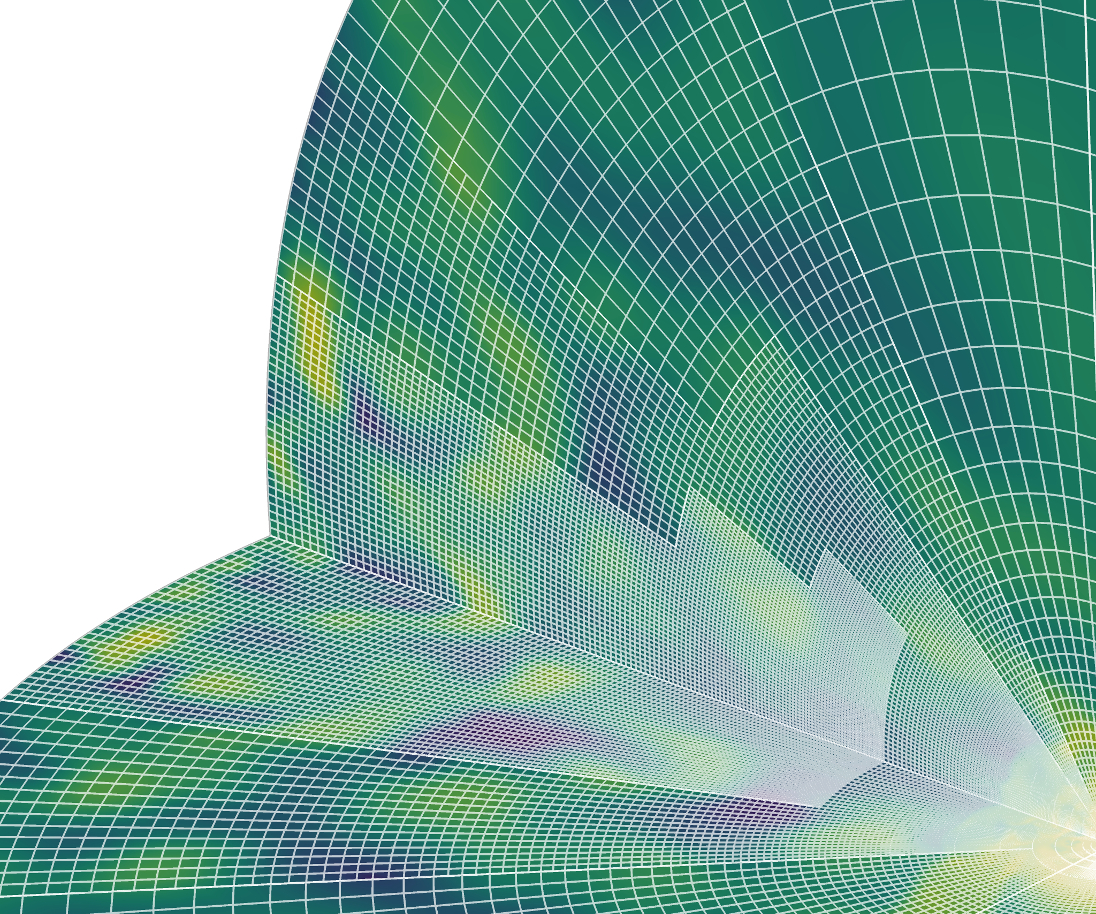
\includegraphics[height=7cm]{Figures/mesh.jpeg}	
\end{subfigure}
\caption{(\textit{left}) Principle of the clumpy wind accretion simulations : we inject into the simulation space (upper right insert) a wind whose micro-structure has been computed out of radiative HD simulations by \cite{Sundqvist2017}. (\textit{right}) Two-slices representation of the upstream hemisphere of the simulation space, with the wind coming from the upper left. We overlaid a logarithmic density map to show the typical size of the inhomogeneities to resolve. The accretor lies in the bottom right corner.}
\label{fig:config_SgXB_and_mesh}
\end{figure}

\indent Since the beginning of my postdoctoral activity two years ago, I started to consider more realistic internal structure for the incoming wind in SgXB than the uniform flow I had worked with during my PhD. Indeed, the line-driven winds of massive stars are notoriously inhomogeneous, due to the line-deshadowing instability \citep{Owocki1984a} which leads to the formation of internal shocks. The serendipituous accretion of these overdense regions, or clumps, has been suggested as a possible explanation to the time variability of the X-ray luminosity in SgXB, of the order of 100 peak-to-peak. Using a two-dimensional pseudo-planar grid sampling a restricted angular region, \cite{Sundqvist2017} recently managed to compute the micro-structure of the wind and by then, the dimensions of the clumps, for an isolated massive stars. To evaluate the impact of clumps on the accretion process, I plunged a compact object in the wind ("CO" in the left panel in Figure\,\ref{fig:config_SgXB_and_mesh}), at different orbital separations, and injected the corresponding wind computed by \cite{Sundqvist2017} within the simulation space (right panel in Figure\,\ref{fig:config_SgXB_and_mesh}). By coupling the stretching of the mesh to the Adaptive Mesh Refinement (AMR) of \texttt{MPI-AMRVAC}, I could design 3D spherical setups spanning several orders of magnitude at an affordable computational cost and resolve small scale off-centered features like clumps injected from the upstream hemisphere. In \cite{ElMellah}, we were able to follow the clumps as they cross the shock and to monitor the time variability at the inner border of the simulation space, corresponding approximately to the dimensions of the NS magnetosphere. With this work, we discovered how tempering the shock could be, which led to variations of the inner mass accretion rate an order of magnitude smaller than the observed variations of the X-ray luminosity in these systems. Thus, if the stochastic variations at low X-ray luminosity seem to match the variability induced by the clumps alone, the high luminosity levels can only be reached due to other underlying mechanisms, possibly within the NS magnetosphere \citep[eg the propeller effect,][]{Bozzo2016}. Concerning the column density levels, we retrieve average values compatible with what has been observed recently in Vela X-1 by \cite{Grinberg2017}. However, in the latter paper, I evaluated the time variability associated to unaccreted clumps passing by the line-of-sight and concluded that this type of micro-structure within the wind can not explain by itself the variations in column density observed by \cite{Grinberg2017}.\\ \\
\indent In \cite{Xia2017}, I carried out a numerical validation of the stretched grid implementation I had made during my PhD by confronting quantitative simulation results of Bondi spherical accretion to the analytical expectations on the mass accretion rate and the location of the sonic point for different adiabatic indexes. We also studied the propagation of a trans-Alv\'enic wind from the solar surface to the Earth orbit to validate the compatibility of the stretched grid with the magneto-HD solver and Powell's method for the cleaning of the divergence of the magnetic field.\\ \\

\subsection*{Project outline}

In X-ray binaries, the challenge of scales can be alleviated thanks to the different dominant physical effects at stake at different scales. For instance, the magnetic field has generally little influence at the orbital scale but is decisive to fully appreciate the conditions in which the accreted flow emits most of the light we observe. Besides, in SgXB, the magnetic field dominates the last phase of accretion possibly through magnetic gating. It is also a key-ingredient of the ejection mechanisms responsible for self-collimated jets we often observe in accreting systems.

\subsubsection*{RLOF discs}

\begin{wrapfigure}{r}{7.2cm}
\vspace*{-1.5cm}
\hspace*{0.1cm}
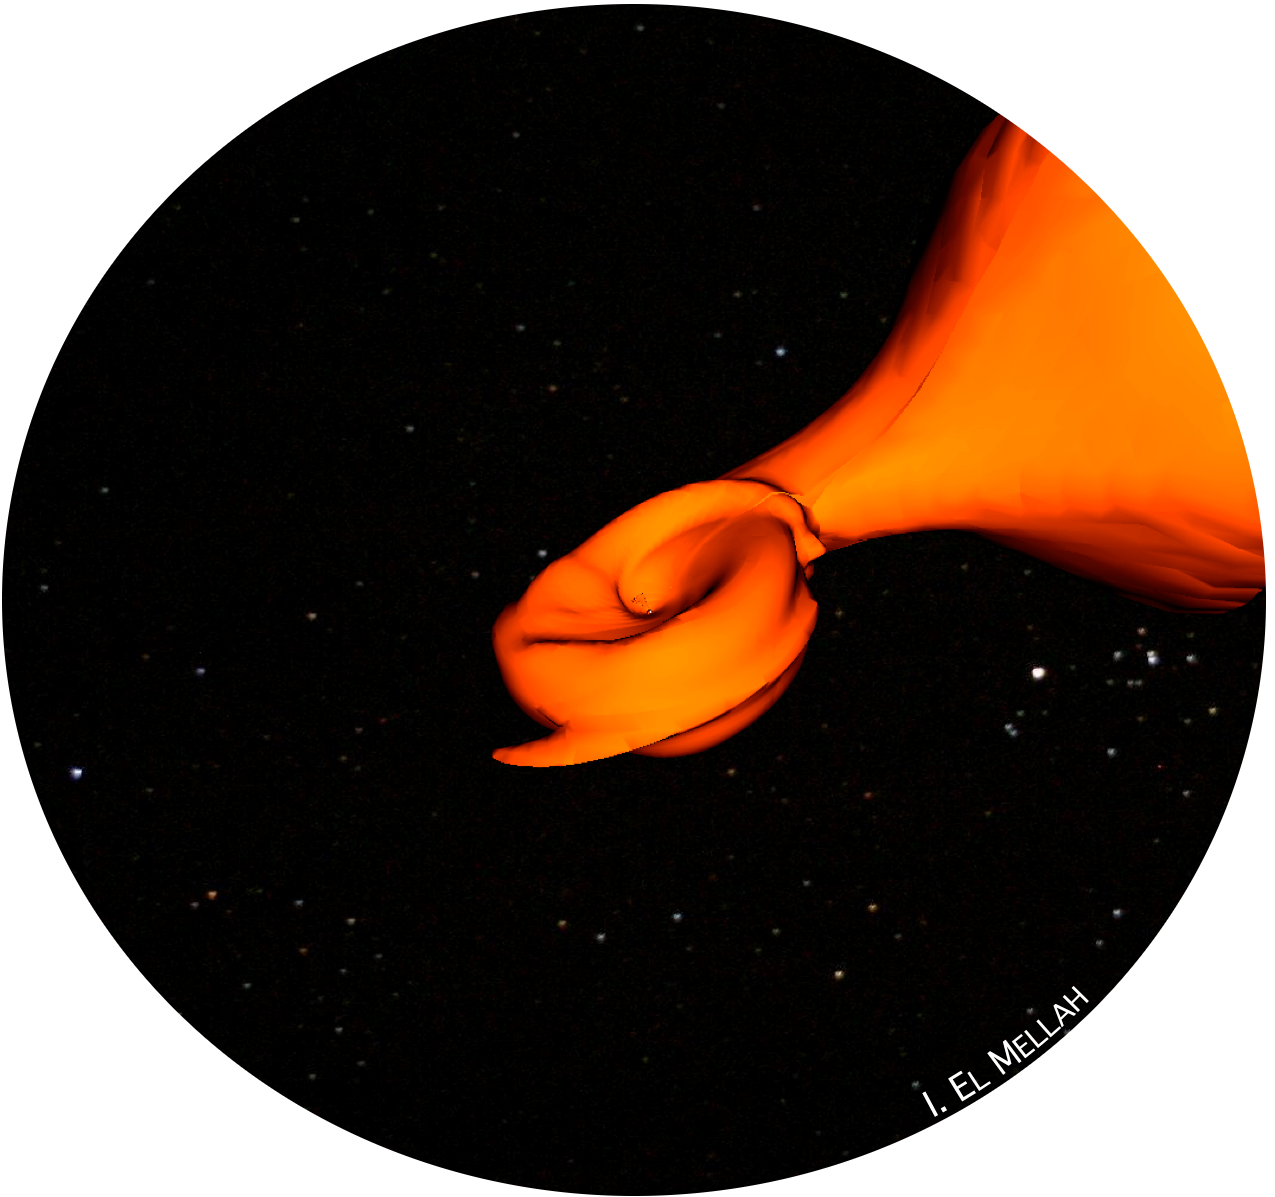
\includegraphics[height=7.1cm]{Figures/RLOF.png}
\caption{Isodensity surface of a 3D flow from a stellar companion (upper right) to an accretor, 1,000 times smaller than the orbital separation between the two bodies.}
\label{fig:bow2.5d}
\end{wrapfigure} 

To guarantee that we work with physically consistent accretion discs, I am now performing numerical simulations of RLOF configurations where the expanded atmosphere of the donor star is channeled into the Roche lobe of the accretor through the first Lagrangian point. This model includes a proxy on viscosity, similar to the one introduced by \cite{Shakura1973}, and energy losses through radiative cooling. The former stands for the turbulent viscosity associated to the magnetic rotational instability \citep{Balbus1991}. Together with spiral shocks, they participate to the evacuation of angular momentum which makes the accretion possible. The ballistic solution is then superseded by the actual formation of a disc around the accretor. Since the plasma largely exceeds 10,000K during the accretion process, a significant fraction of the elements is ionized. We make use of the SPEX cooling tables for solar abundances to compute the cooling function \citep{VanMarle2011}, which yields cooling rates large enough to impact the thickness of the flow. However, the numerically convenient optically thin assumption we currently make breaks up in the disc and must be complemented with a flux-limited diffusion method I plan to implement in \texttt{MPI-AMRVAC}. These improvements could first lead to insights concerning the origin of negative superhumps in cataclysmic variables \citep[CV, ][]{Murray1998}. Replacing the inner accretor with a BH or a lowly magnetized NS, the wrapping of the disc could also be studied and numerical results obtained in the context of Smooth Particle Hydrodynamics simulations could be confronted \citep{Foulkes2006}. If the disc turns out to be misaligned with the orbital plane, it could have a serious impact on jet-launching conditions since a misalignement with the BH spin is likely to induce a precession of the jets \cite{Liska2017}.
  
\subsubsection*{Diving into the magnetosphere}

\indent Once I obtain a satisfying self-generated RLOF disc, I will use it as a fruitful landscape to explore two kinds of systems. First, with Zakaria Meliani, we wish to make this setup a scaled up version of a NS accretor in a Low Mass X-ray binary. A magnetized white dwarf (WD) in a CV intermediate polar alleviates the contrast between the orbital separation and the size of the compact object, while still retaining most of the geometry of the system: a RLOF donor star feeding a disc truncated in its innermost regions by the magnetic field of the accretor \citep{Ghosh1977}. Until now, the studies which have been carried on make an adiabatic assumption to bypass the question of cooling \citep{Ju2017}. Working with a physically-motivated vertical profile of the disc, we think we can shed light on the question of the spin-down efficiency of the accretion process on the WD. We would also be in possession of a reliable tool to elucidate the disc reformation during the afterglow phase of novas \citep{Ness2012}.\\ \\
\indent This twofold setup also serves another purpose : diving into the magnetosphere of an accreting NS. Numerically, we recently implemented and validated a method of magnetic splitting generalized to non-potential fields \citep{Xia2017}. It enables us to handle more accurately the magnetic field evolution, in particular in low-$\beta$ shock-dominated plasmas, and to clean more easily the non-zero divergence. With this new feature available, we want to study how the innermost parts of the wind accreted flow derived in \cite{ElMellah} behave. Is the angular momentum carried by the clumps large enough to form a transient disc-like structure or does the NS magnetic field come into play before they can do so? The possible magnetic gating undergone by the innermost parts of the flow has never been explored with physical inputs accounting for the upper scales. Hence, it has produced fruitful results but ambiguous since the prescriptions employed have been independent from the large scale parameters (such as the stellar ones). We also want to address the case where the NS magnetospheric radius is much larger, of the order of the accretion radius. How does it alter the shock?  \\ \\

%\newpage

To conclude, the numerical expertise I have developed in Computational Astrophysics enables me to make the most of the high performance computing technologies available. They have ushered in a particularly exciting period to address a wide range of questions pertaining to accretion in X-ray binaries. To progress on these questions, I need to keep connecting with observers and modelers in this field, both communities being represented in Potsdam : with researchers from the Max Planck Institute for Gravitational Physics, I could reinforce the modeling of the relativistic surroundings of the accretor, where the X-rays we observe are produced, while the expertise in stellar Astrophysics at the Institut für Physik und Astronomie would provide a more realistic representation of the stellar wind which feeds the accretor. The conjunction of these two features supplies a unique opportunity to bridge the gap between the stellar and wind properties on one hand, and the high energy phenomena at stake near the compact object on the other hand. High energy Astrophysics is also a domain of interest of the Leibniz Institute for Astrophysics where quasars, a type of supermassive black holes undergoing an intense accretion phase, are under investigation. I already showed my capacity to obtain external fundings and do intend to raise the funds necessary to such a project with applications to ERC grants and to programs sponsored by the Deutsche Forschungsgemeinschaft. Beyond their autonomous requirements and satisfactions, I also expect my teaching duties to be opportunities to arouse the interest of the students in pursuing in this research domain. Should it be the case, I would gladly mentor them, as I have been mentored on my way to the endlessly mesmerizing field of Astrophysics. 

%\indent More generally, the B field opens the door to a wide range of accretion-ejection mechanisms in the disc itself (Blandford-Payne 82, Casse 04), provided we have a physically-motivated disc thickness profile (see previous section). Transition from jet emitting discs to standard accretion discs (SS75) as a possible explanation for the two states observed in LMXB (Ferreira 06).\\ \\

%\section*{Conclusion}
%
%Bedrock model 
%
%Longer term prospective

\newpage

%\newgeometry{left=2cm,right=2cm,top=2.5cm,bottom=2.5cm}
\setlength{\bibsep}{5pt}
\small
\bibliographystyle{agsm}
\bibliography{/Users/Ileyk/Documents/Bibtex/research_statement_no_url}

\newpage

\phantom{n}

\end{document}
%%%%%%%%%%%%%%%%%  Fin du fichier Latex  %%%%%%%%%%%%%%%%%%%%%%%%%%%%%%

